If scientific computing lives at the Linux command line,
then being a Windows users can be tricky.
The two parts of our workflow that are most difficult to implement on Windows
are executing Makefiles and creating symbolic links.

There are a variety of ways to run Make.
Covert and Sweeney 
\href{https://github.com/rlsweeney/public_cs_texas/blob/master/README.md}{suggest}
using
\href{https://chocolatey.org/install}{Chocolatey}.
This entry describes how to use GitBash to run Make.

We are only aware of one way to get Windows
to create symbolic links using \texttt{ln -s}.
(Windows typically uses a distinct \texttt{mklink} syntax).
It employs GitBash and is described below.

\subsection{Install GitBash}
Download and install GitBash here from
\url{https://git-scm.com/downloads}
\begin{itemize}
    \item Please make sure to pick ``commit Unix-style line endings''
    \begin{figure}[H]
        \centering
        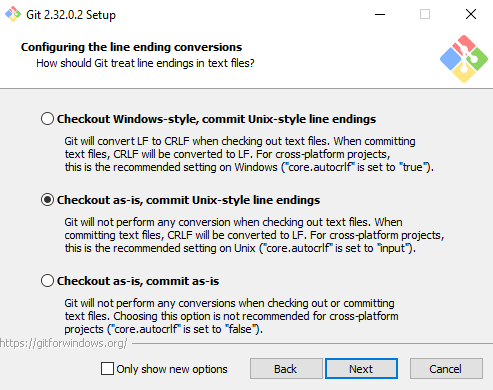
\includegraphics[width=0.5\textwidth]{figures/workflow/make_on_win_gitbash_screenshot1.png}
    \end{figure}
    \item Please also check enable symbolic links (should be checked by default)
    \begin{figure}[H]
        \centering
        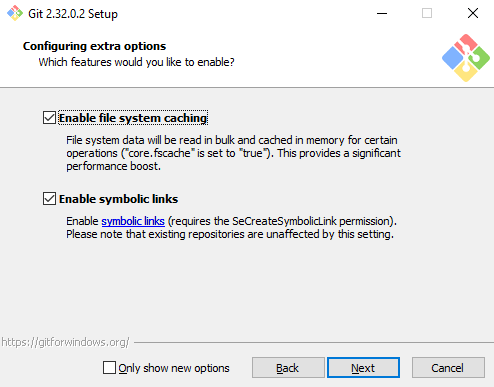
\includegraphics[width=0.5\textwidth]{figures/workflow/make_on_win_gitbash_screenshot2.png}
    \end{figure}
\end{itemize}


\subsection{Install \texttt{make}}
Source: \url{https://gist.github.com/evanwill/0207876c3243bbb6863e65ec5dc3f058#make}
\begin{enumerate}
    \item Go to ezwinports (\url{https://sourceforge.net/projects/ezwinports/files/}).
    \item Download \texttt{make-4.1-2-without-guile-w32-bin.zip} (get the version without guile).
    \item Extract zip.
    \item Copy the contents to your \texttt{Git{\textbackslash}mingw64{\textbackslash}} merging the folders,
        but do NOT overwrite/replace any existing files.
\end{enumerate}

\subsection{Install \texttt{wget}}
Source: \url{https://gist.github.com/evanwill/0207876c3243bbb6863e65ec5dc3f058#wget}
\begin{enumerate}
    \item Download the lastest wget binary for windows from eternallybored
        (\url{https://eternallybored.org/misc/wget/});
        they are available as a zip with documentation, or just an exe.
    \item If you downloaded the zip, extract all (if windows built in zip utility gives an error, use 7-zip).
    \item Rename the file \texttt{wget64.exe} to \texttt{wget.exe} if necessary.
    \item Move wget.exe to your \texttt{Git{\textbackslash}mingw64{\textbackslash}bin{\textbackslash}}.
\end{enumerate}

\subsection{Create symbolic links on Windows using \texttt{ln -s}}
To do so, you need to run GitBash as Administrator
    (instructions to \textit{always} run GitBash as Administrator are the end).

\noindent \textit{NOTE}: 
Executing the steps below will overwrite
the default behavior of \texttt{ln} on GitBash.
\begin{enumerate}
\item Open GitBash
\item
\begin{lstlisting}[language=bash]
cd ~
echo 'export MSYS=winsymlinks:nativestrict' >> .bash_profile
echo 'export MSYS=winsymlinks:nativestrict' >> .bashrc
\end{lstlisting}
\item Close all GitBash windows.
\end{enumerate}
Technically, you should only have to edit either
\texttt{.bash\_profile} or \texttt{.bashrc},
but sources differ and experiences differ.
Anyway, it won't hurt to do both.

\subsubsection{Optional: Always run GitBash as Administrator}
Source: \url{http://pinter.org/archives/6129} \\
\noindent \textit{NOTE}: Only the part mentioned below is needed.
\begin{enumerate}
    \item Click the Windows Start button and type Git Bash
    \item Right-click the found link and select ``Open file location''
    \item Right-click the menu shortcut and select ``Properties''
    \item On the ``Compatibility'' tab, check the box ``Run this program as an administrator''.
    \item Click ``OK'' at the bottom
\end{enumerate}
